\documentclass[conference]{IEEEtran}

\usepackage[T1]{fontenc}
\usepackage[utf8]{inputenc}
\usepackage{cite}
\usepackage{amsmath,amssymb}
\usepackage{booktabs}
\usepackage{array}
\usepackage{url}
\usepackage{graphicx}
\usepackage{tikz}
\usepackage{algorithm}
\usepackage{algpseudocode}
\usepackage{xcolor}
\usepackage{balance}
\usetikzlibrary{arrows.meta,positioning,fit,shapes.geometric,backgrounds}

\title{LAWRENCE: A Local-First Parallel-Facet Assistant\\for Contextual Reasoning, Durable Memory, and Edge-Resident Interaction}

\author{
\IEEEauthorblockN{Project Technical Article}
\IEEEauthorblockA{LAWRENCE v0.1 Architecture Description}
}

\begin{document}
\maketitle

\begin{abstract}
This paper presents LAWRENCE, a local-first assistant architecture designed to function as an actual contextual companion rather than a stateless chatbot. The system is intended for edge-resident operation on modest hardware, with privacy-preserving defaults, durable Markdown memory, and replaceable inference backends. LAWRENCE is organized as one assistant kernel that constructs a frozen context snapshot and dispatches multiple internal facets in parallel: current-context interpretation, memory recall, journaling and distillation, tool planning, web retrieval, fast reasoning, slow reasoning, and merge arbitration. The result is a system that can answer immediately, continue thinking after the first response, and grow long-term memory without hiding that memory inside opaque storage. This article introduces the project from first principles, explains why a watcher-style assistant requires a different architecture than a prompt-response chatbot, and details the implementation model spanning user interaction, multimodal capture, memory formation, retrieval, provider routing, workflow integration, and privacy control. The paper also provides diagrams, data contracts, and pseudocode to make the system understandable to readers who are new to the project.
\end{abstract}

\begin{IEEEkeywords}
local-first AI, multimodal assistant, edge inference, contextual retrieval, Zettelkasten memory, agent orchestration, privacy-aware systems, workflow integration
\end{IEEEkeywords}

\section{Introduction}
The prevailing shape of conversational AI software is still the request-response chatbot. A user writes a prompt, the system optionally retrieves context, calls a model, and returns text. This pattern is adequate for isolated question answering, but it breaks down when an assistant is expected to stay aware of the user's environment, remember ongoing work, respond through voice, and build an inspectable long-term record of what happened. A serious assistant needs continuity, not merely clever one-shot completion.

LAWRENCE is built to address that gap. The name stands for \emph{Local Agentic Watcher Reasoning on Edge Node Contextualizing Engine}. The wording is deliberate. The system is \emph{local} because the default assumption is that inference and storage happen on the user's own machine. It is \emph{agentic} because the assistant can propose or later execute tool-mediated actions. It is a \emph{watcher} because it pays attention to the user's current digital environment instead of waiting to be spoon-fed every relevant fact. It performs \emph{reasoning} because some questions require more than immediate retrieval or pattern matching. It operates at the \emph{edge} because the hardware target is modest and personal, not a remote cluster. Finally, it is a \emph{contextualizing engine} because its main job is to turn raw, transient activity into coherent context.

The project does not assume that one large model invocation can perform all of these jobs well. LAWRENCE instead treats assistance as a coordination problem among multiple specialized internal processes with different latencies, duties, and failure modes. This is the paper's central thesis: a practical personal assistant should be modeled as one kernel with many simultaneous evidentiary organs, not as one serial pipeline or one permanent monologue.

This article introduces the project step by step for readers who have not seen the repository or prior planning discussions. It explains what problem LAWRENCE tries to solve, what conceptual model governs the system, why the memory substrate is Markdown-based, how the fast and slow loops cooperate, what implementation choices have been made, and where the architectural boundaries lie.

\subsection{What This Paper Contributes}
This paper makes four project-specific contributions.

\begin{enumerate}
\item It defines LAWRENCE as a \emph{watcher-assistant} rather than a conventional chatbot.
\item It formalizes the \emph{parallel-facet} execution model used by the assistant kernel.
\item It describes a \emph{Markdown-first durable memory fabric} that keeps long-term memory inspectable and portable.
\item It specifies a \emph{local-first modular implementation architecture} using replaceable model runtimes, workflow connectors, and policy controls.
\end{enumerate}

\section{Why Another Assistant Architecture Is Needed}
Most assistant demos fail at one of three points. First, they are temporally shallow: they answer the current prompt but do not preserve coherent memory of what has been happening. Second, they are operationally fragile: the moment the primary model call is slow or unavailable, the whole user experience stalls. Third, they are opaque: whatever context they retain is trapped inside session buffers, vector stores, or cloud logs that the user does not really own.

For a local-first assistant meant to live with the user over time, those weaknesses are structural rather than cosmetic. Consider a concrete scenario. A user is switching between code, documentation, browser tabs, and voice notes. The assistant should be able to tell that the user is working on the same topic even when the surface modality changes. It should be able to answer a quick question immediately, log the activity in the background, remember that an earlier task is related, and later synthesize a clearer explanation or reminder. If the assistant waits for one large serial pipeline to complete, the experience will feel slow and brittle. If it remembers only through a hidden cache, the user will not trust or understand it. If it depends on a remote provider by default, it will violate the project's local-control goal.

LAWRENCE therefore starts from a different assumption: useful assistance comes from coordinating multiple partial views of the user's situation. Some of those views are immediate, some are historical, some are internal, and some are optional outward branches such as web retrieval or tool use. The project is about organizing those views into one coherent assistant.

\section{From Chatbot to Watcher-Assistant}
The word ``watcher'' can sound abstract or even suspicious unless it is carefully defined. In LAWRENCE, a watcher is not a surveillance system and not an always-record-everything black box. A watcher is a local subsystem that notices relevant changes in the user's environment and converts them into context. The point is not to archive all raw data forever. The point is to make the assistant situationally aware enough to be helpful.

The watcher-assistant idea can be explained through a simple progression.

\begin{enumerate}
\item A user is working in an application, browsing, writing, or speaking.
\item The system observes lightweight context signals such as active window state, a low-cost screen sample, or speech activity.
\item A meaningful trigger occurs: a hotkey, a voice command, a typed query, or a detectable context change.
\item The system freezes a turn snapshot so that all internal subsystems reason about the same moment.
\item Multiple facets operate over that snapshot in parallel.
\item The user receives an immediate answer as soon as enough evidence exists.
\item The system continues to refine, log, and write memory after the first answer.
\end{enumerate}

This progression is important because it makes the project intelligible. LAWRENCE is not ``chat plus memory'' and not ``an LLM with tools.'' It is a contextual runtime that uses conversation as one surface among several.

\section{Design Requirements and Boundaries}
The architecture follows a set of project requirements that constrain all subsystem choices.

\subsection{Local-First Execution}
The system should prefer local inference and local storage by default. Cloud providers may be used later as optional fallbacks or convenience modes, but the assistant must not become unusable without them. This is both a privacy requirement and a robustness requirement.

\subsection{Modest Edge Hardware}
The project assumes hardware closer to a personal workstation than to a server. That means the system must treat compute as scarce. Large always-on pipelines, heavy unbounded recursion, or full-resolution visual analysis on every frame would be irresponsible design choices.

\subsection{Durable Human-Readable Memory}
Long-term memory must be inspectable by the user. The canonical store is therefore linked Markdown in a Zettelkasten-like form. Auxiliary caches and indexes are allowed, but they do not replace the durable record.

\subsection{Parallel Internal Work}
The assistant must remain responsive while background processes continue to think, retrieve, or write. This requirement directly motivates the fast-loop/slow-loop split and the parallel-facet runtime.

\subsection{Privacy and Human Confirmation}
The assistant is expected to see sensitive context. For that reason, screen capture, microphone capture, outbound cloud calls, web access, and system-control actions must be policy-mediated. Tool execution is not permitted to become a hidden side effect.

\subsection{Non-Goals}
LAWRENCE is not designed as an enterprise compliance platform, a benchmark-focused agent arena, or a maximal automation engine that silently acts on behalf of the user. It is a personal-use-first assistant substrate.

\section{Conceptual Model of LAWRENCE}
The cleanest way to understand LAWRENCE is to separate four levels of the system: interaction surfaces, the assistant kernel, supporting fabrics, and controlled outward branches.

\begin{itemize}
\item \textbf{Interaction surfaces} are what the user touches: voice, text, overlays, and hotkeys.
\item \textbf{The assistant kernel} owns turn creation, facet dispatch, arbitration, and delivery.
\item \textbf{Supporting fabrics} are the context fabric and memory fabric that provide shared state and durable knowledge.
\item \textbf{Outward branches} are optional subsystems such as web retrieval, workflows, and tools that the kernel may use when policy allows.
\end{itemize}

Figure~\ref{fig:architecture} shows the full architecture.

\begin{figure*}[t]
\centering
\resizebox{\textwidth}{!}{%
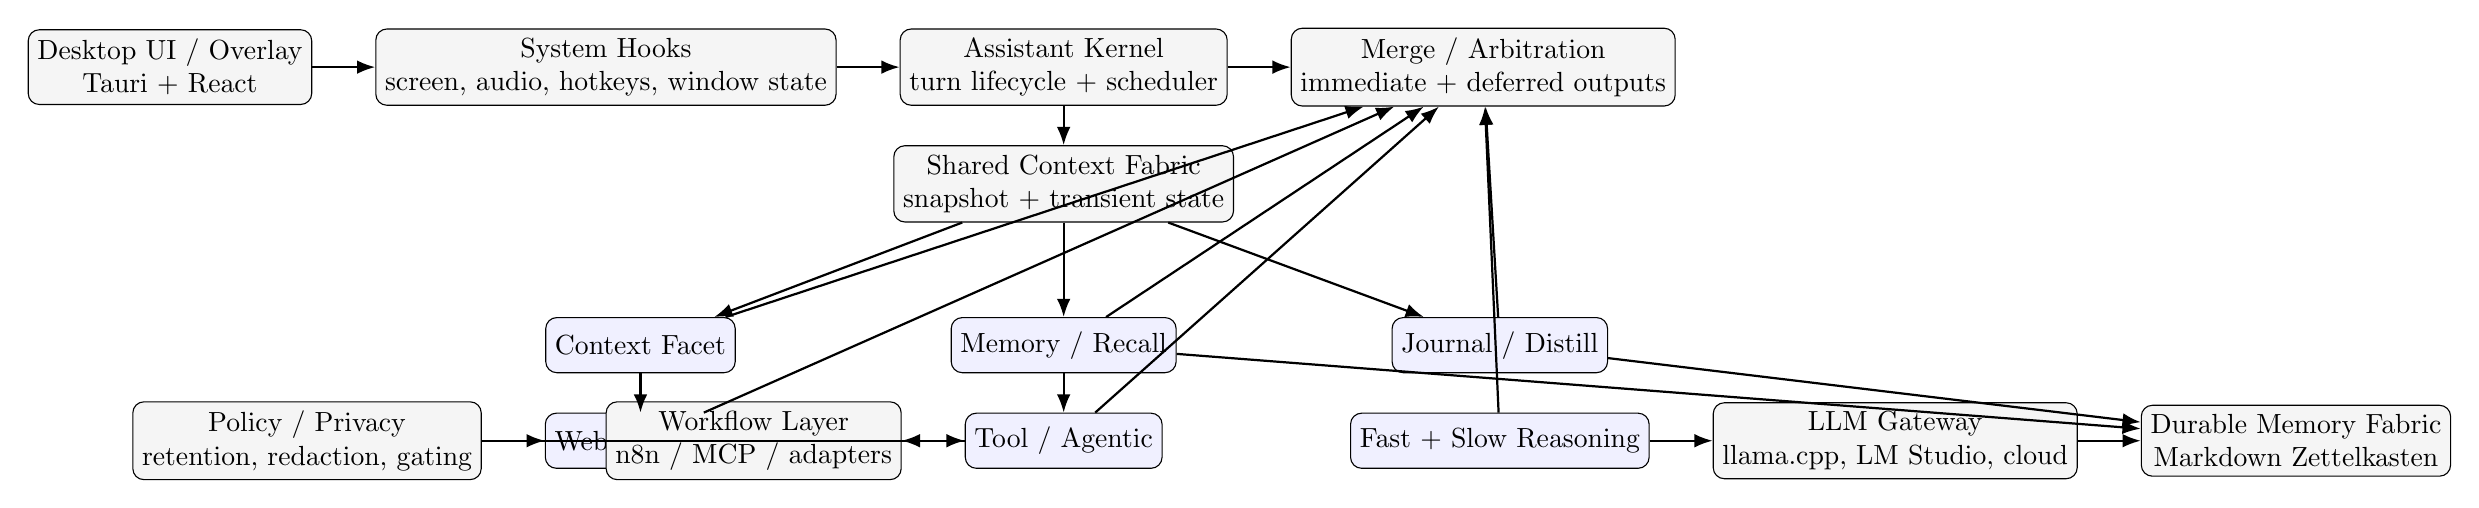
\begin{tikzpicture}[
  node distance=5mm and 8mm,
  box/.style={draw, rounded corners, align=center, minimum height=8mm, minimum width=24mm, fill=gray!8},
  facet/.style={draw, rounded corners, align=center, minimum height=7mm, minimum width=22mm, fill=blue!6},
  arrow/.style={-Latex, thick}
]
\node[box] (ui) {Desktop UI / Overlay\\Tauri + React};
\node[box, right=of ui] (hooks) {System Hooks\\screen, audio, hotkeys, window state};
\node[box, right=of hooks] (kernel) {Assistant Kernel\\turn lifecycle + scheduler};
\node[box, right=of kernel] (merge) {Merge / Arbitration\\immediate + deferred outputs};
\node[box, below=of kernel] (fabric) {Shared Context Fabric\\snapshot + transient state};

\node[facet, below left=12mm and 20mm of fabric] (context) {Context Facet};
\node[facet, below=12mm of fabric] (memory) {Memory / Recall};
\node[facet, below right=12mm and 20mm of fabric] (journal) {Journal / Distill};
\node[facet, below=of context] (web) {Web Retrieval};
\node[facet, below=of memory] (tools) {Tool / Agentic};
\node[facet, below=of journal] (reason) {Fast + Slow Reasoning};

\node[box, left=of web] (policy) {Policy / Privacy\\retention, redaction, gating};
\node[box, right=of reason] (gateway) {LLM Gateway\\llama.cpp, LM Studio, cloud};
\node[box, left=of tools] (n8n) {Workflow Layer\\n8n / MCP / adapters};
\node[box, right=of gateway] (memoryvault) {Durable Memory Fabric\\Markdown Zettelkasten};

\draw[arrow] (ui) -- (hooks);
\draw[arrow] (hooks) -- (kernel);
\draw[arrow] (kernel) -- (merge);
\draw[arrow] (kernel) -- (fabric);
\draw[arrow] (fabric) -- (context);
\draw[arrow] (fabric) -- (memory);
\draw[arrow] (fabric) -- (journal);
\draw[arrow] (context) -- (merge);
\draw[arrow] (memory) -- (merge);
\draw[arrow] (journal) -- (merge);
\draw[arrow] (web) -- (merge);
\draw[arrow] (tools) -- (merge);
\draw[arrow] (reason) -- (merge);
\draw[arrow] (context) -- (web);
\draw[arrow] (memory) -- (tools);
\draw[arrow] (journal) -- (memoryvault);
\draw[arrow] (policy) -- (web);
\draw[arrow] (policy) -- (tools);
\draw[arrow] (reason) -- (gateway);
\draw[arrow] (tools) -- (n8n);
\draw[arrow] (memory) -- (memoryvault);
\draw[arrow] (gateway) -- (memoryvault);
\end{tikzpicture}
}
\caption{System architecture of LAWRENCE. The assistant kernel sits between interaction surfaces and internal facets, while policy, workflows, providers, and durable memory remain explicit subsystems.}
\label{fig:architecture}
\end{figure*}

The architecture has one especially important property: the kernel is singular, but the inner work is plural. This is how the project remains coherent without becoming monolithic.

\subsection{Why One Kernel?}
Using one kernel gives the project a single place where turns are defined, context versions are assigned, policies are applied, and outputs are merged. Without that anchor, the system would fragment into loosely related mini-agents that each maintain their own view of the user's state.

\subsection{Why Many Facets?}
Using multiple facets acknowledges that not all work has the same shape. Retrieval is not the same as journaling. Tool planning is not the same as immediate conversational continuity. Slow synthesis is not the same as low-latency answer generation. Treating these as separate evidence producers makes the overall assistant more resilient and easier to reason about.

\section{Interaction Surfaces and User Experience}
LAWRENCE uses audio and text as the primary conversation surfaces. This design follows the intended use case: the assistant should be available during actual work, not only when the user decides to sit inside a chat pane. Voice supports ambient interaction. Text supports precision, structured instructions, code, and searchable records.

Visual capture is deliberately secondary. The system is not a screen-native chat interface with a little bit of memory attached. Instead, the screen is one contextual modality among several. It helps the assistant understand what the user is doing, but it does not replace the main audio-plus-text interaction loop.

The intended user-visible surfaces are:

\begin{itemize}
\item a hotkey-triggered overlay,
\item text input and streamed text output,
\item voice input and spoken response,
\item low-frequency contextual suggestions,
\item deferred addenda when the slow loop finishes better work.
\end{itemize}

This leads to a user experience where the assistant can be helpful in stages rather than pretending every answer arrives fully formed in one shot.

\section{Context Capture and Snapshot Construction}
The assistant's context model is built around \emph{frozen turn snapshots}. Whenever a meaningful event occurs, the kernel captures a stable reference frame for internal processing. The snapshot is not meant to contain every raw detail. Instead, it acts as the turn's index into current evidence.

The core snapshot contract is:

\begin{equation}
\label{eq:snapshot}
\begin{aligned}
\mathrm{TurnContextSnapshot} = \{&
\text{turn\_id}, \text{ts}, \text{trigger\_type}, \text{user\_query},\\
&\text{screen\_ref}, \text{audio\_ref}, \text{thread\_ref}, \text{app\_ref},\\
&\text{time\_ref}, \text{reminder\_ref}, \text{latest\_chat\_refs},\\
&\text{policy\_state}, \text{context\_version}\}
\end{aligned}
\end{equation}

This representation has three purposes.

\begin{enumerate}
\item It gives all internal facets the same point of departure.
\item It allows stale late-arriving outputs to be discarded by comparing \emph{context\_version} values.
\item It makes evidence provenance explicit for later audit, journaling, and debugging.
\end{enumerate}

\subsection{Screen Strategy}
On modest hardware, continuous full-resolution visual understanding is the wrong baseline. LAWRENCE therefore treats the screen as a selectively sampled signal. A lightweight observer can run at higher frequency to detect material change. When the system sees that the working context has shifted, it can capture a richer frame and metadata for deeper interpretation. Basic OCR may exist, but the system is not built on the assumption that OCR text alone explains the user's situation.

\subsection{Audio Strategy}
Audio serves both as a direct command surface and as an environmental context source. With always-listening mode enabled, LAWRENCE may transcribe or tag speech activity using a lightweight speech-to-text stack such as Whisper-derived systems \cite{radford2022whisper}. Trigger phrases, hotkeys, or command-like utterances can then escalate to a full turn. Non-trigger audio does not need to launch deep reasoning every time; it can instead feed journaling or short-term contextual state.

\subsection{Temporal and Thread Context}
A meaningful assistant needs more than raw media. LAWRENCE also models time, thread continuity, stale versus active contexts, recent chat history, and reminder-like structures where available. Even before full external integrations exist, temporal inference is essential because many assistant tasks are really about continuity: what was being worked on, what is overdue, what is still open, and what is likely to matter next.

\section{The Parallel-Facet Runtime}
The defining runtime decision in LAWRENCE is that a turn does not move through a single serial pipeline. Instead, the kernel launches several internal facets at once and lets them produce evidence under deadlines. This is the part of the system most likely to be misunderstood, so it deserves careful explanation.

In a serial assistant, the system would first capture context, then retrieve, then reason, then maybe call tools, then maybe log memory. That looks simple on a whiteboard but creates avoidable latency and failure propagation. If one stage is slow, everything waits. If one stage fails, the whole turn becomes brittle. LAWRENCE avoids this by turning each major responsibility into a facet that operates over the same frozen snapshot.

Figure~\ref{fig:lifecycle} shows the turn lifecycle.

\begin{figure*}[t]
\centering
\resizebox{\textwidth}{!}{%
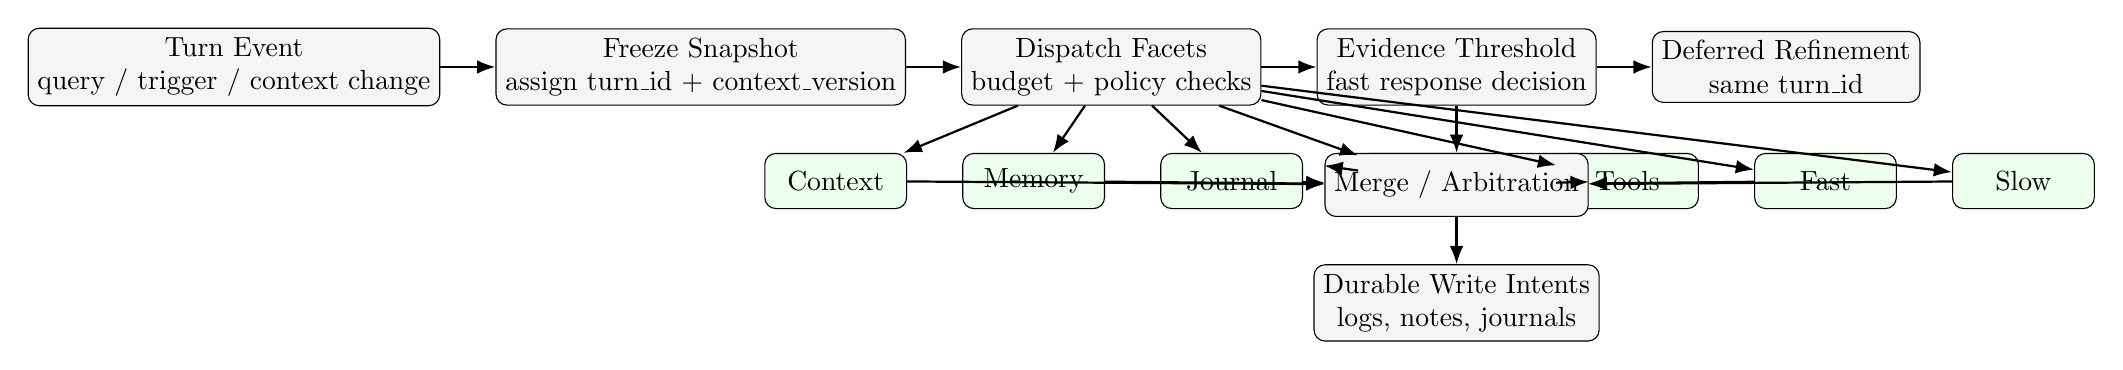
\begin{tikzpicture}[
  node distance=6mm and 7mm,
  phase/.style={draw, rounded corners, minimum width=24mm, minimum height=8mm, align=center, fill=gray!8},
  facet/.style={draw, rounded corners, minimum width=18mm, minimum height=7mm, align=center, fill=green!7},
  arrow/.style={-Latex, thick}
]
\node[phase] (event) {Turn Event\\query / trigger / context change};
\node[phase, right=of event] (snap) {Freeze Snapshot\\assign turn\_id + context\_version};
\node[phase, right=of snap] (dispatch) {Dispatch Facets\\budget + policy checks};
\node[phase, right=of dispatch] (threshold) {Evidence Threshold\\fast response decision};
\node[phase, right=of threshold] (deferred) {Deferred Refinement\\same turn\_id};

\node[facet, below=of dispatch, xshift=-35mm] (f1) {Context};
\node[facet, right=of f1] (f2) {Memory};
\node[facet, right=of f2] (f3) {Journal};
\node[facet, right=of f3] (f4) {Web};
\node[facet, right=of f4] (f5) {Tools};
\node[facet, right=of f5] (f6) {Fast};
\node[facet, right=of f6] (f7) {Slow};

\node[phase, below=of threshold] (merge) {Merge / Arbitration};
\node[phase, below=of merge] (write) {Durable Write Intents\\logs, notes, journals};

\draw[arrow] (event) -- (snap);
\draw[arrow] (snap) -- (dispatch);
\draw[arrow] (dispatch) -- (threshold);
\draw[arrow] (threshold) -- (deferred);
\draw[arrow] (dispatch) -- (f1);
\draw[arrow] (dispatch) -- (f2);
\draw[arrow] (dispatch) -- (f3);
\draw[arrow] (dispatch) -- (f4);
\draw[arrow] (dispatch) -- (f5);
\draw[arrow] (dispatch) -- (f6);
\draw[arrow] (dispatch) -- (f7);
\draw[arrow] (f1) -- (merge);
\draw[arrow] (f2) -- (merge);
\draw[arrow] (f3) -- (merge);
\draw[arrow] (f4) -- (merge);
\draw[arrow] (f5) -- (merge);
\draw[arrow] (f6) -- (merge);
\draw[arrow] (f7) -- (merge);
\draw[arrow] (threshold) -- (merge);
\draw[arrow] (merge) -- (write);
\end{tikzpicture}
}
\caption{Turn lifecycle in LAWRENCE. Immediate response generation and deferred refinement coexist with journaling and durable write preparation instead of waiting for a serial pipeline to finish.}
\label{fig:lifecycle}
\end{figure*}

\subsection{Facet Roles}
Each facet has a distinct job.

\begin{itemize}
\item \textbf{Current-context facet}: explains what is happening now from live context signals.
\item \textbf{Memory facet}: retrieves prior notes, linked neighborhoods, thread fragments, and relevant journals.
\item \textbf{Journal facet}: distills transient events into candidate durable records.
\item \textbf{Tool facet}: proposes actions or workflow calls, subject to policy.
\item \textbf{Web facet}: retrieves external evidence and normalizes it as one evidence branch, not as the assistant's source of truth.
\item \textbf{Fast reasoning facet}: produces low-latency conversational continuity.
\item \textbf{Slow reasoning facet}: performs deeper restructuring, critique, and refinement.
\item \textbf{Merge facet}: arbitrates across evidence streams and produces immediate output, deferred output, and durable write intents.
\end{itemize}

\subsection{Fast Loop and Slow Loop}
The fast loop exists because a personal assistant must feel alive. A user should not wait for a perfect answer before getting a useful answer. The slow loop exists because some tasks genuinely require more deliberation. Rather than forcing one loop to imitate the other, LAWRENCE keeps both and lets them cooperate.

This split also clarifies the project's internal \emph{alter-ego} and \emph{main ego} distinction. The alter-ego is not a theatrical second persona. It is the internal structuring intelligence that critiques, balances, and reorganizes candidate responses. The main ego is the visible presentation layer that shapes the final wording and style for the user. The two-layer model is useful precisely because it separates internal reasoning discipline from surfaced tone.

\section{Durable Memory as Linked Markdown}
One of LAWRENCE's strongest architectural commitments is that durable memory should be a file-based, human-readable artifact. This is unusual in AI systems, which often hide memory in opaque stores. LAWRENCE chooses the opposite direction for three reasons.

First, inspectability matters. The user should be able to see what the assistant remembers. Second, portability matters. The memory should outlive any specific runtime or provider. Third, editability matters. Human notes and system-generated notes should be able to coexist in the same durable space.

The memory model follows a Zettelkasten-like structure. Each note has stable metadata and may link to neighboring notes. This allows the memory space to behave like a graph rather than a flat archive.

\begin{table}[t]
\caption{Primary durable note types in LAWRENCE}
\label{tab:noteschema}
\centering
\begin{tabular}{p{0.22\columnwidth} p{0.68\columnwidth}}
\toprule
\textbf{Type} & \textbf{Purpose} \\
\midrule
context\_log & Distilled per-turn or context-change record of what was happening and why it mattered. \\
journal\_daily & Periodic synthesis of ongoing activity, decisions, open loops, and reminders. \\
task\_note & A focused note for user intent, planned actions, blockers, and outcomes. \\
knowledge\_note & A more stable reusable insight or explanation that should be recalled later. \\
\bottomrule
\end{tabular}
\end{table}

The required metadata fields are:

\begin{equation}
\begin{aligned}
\{&\text{id}, \text{type}, \text{created\_at}, \text{updated\_at}, \text{entities},\\
&\text{tags}, \text{links}, \text{source\_refs}, \text{confidence}, \text{privacy\_level}\}
\end{aligned}
\end{equation}

\subsection{Why Markdown Instead of SQL as the Canonical Store?}
SQL or document databases are excellent for indexing and querying, but they are not the right canonical memory representation for this project. A user cannot naturally browse a database as a personal memory vault. Markdown, by contrast, is transparent. The system can still maintain lexical indexes, vector indexes, recency caches, or graph sidecars, but those remain derivative artifacts.

\subsection{Distillation Rather Than Raw Retention}
LAWRENCE does not try to keep all raw screen and audio capture forever. Instead, it keeps transient buffers only as long as needed to support the active turn, journaling, or short-term continuity. After that, raw material is distilled into durable notes. This keeps the memory fabric meaningful and reduces privacy risk.

\subsection{From Logs to Zettels and Journals}
LAWRENCE distinguishes between three related but non-identical durable artifacts: low-level context logs, promoted task or knowledge notes, and periodic journals. Context logs are the first durable landing zone. They capture a distilled description of what happened during a turn or context change. Promoted task and knowledge notes sit above them and represent material that should remain useful after the immediate session. Journals then synthesize multiple notes over a larger time window.

Let $x$ be a transient observation derived from the current turn. LAWRENCE can score its priority for durable promotion using
\begin{equation}
\label{eq:distill}
P_{\mathrm{dist}}(x) =
\alpha_n N(x) + \alpha_s S(x) + \alpha_u U(x) + \alpha_t T(x) + \alpha_a A(x),
\end{equation}
where $N(x)$ is novelty with respect to recent context, $S(x)$ is contextual salience, $U(x)$ is explicit user emphasis, $T(x)$ is thread persistence, and $A(x)$ is actionability or open-loop importance. Each term is normalized to $[0,1]$. A transient item is promoted when $P_{\mathrm{dist}}(x) \ge \tau_{\mathrm{dist}}$, when it is explicitly pinned by the user, or when it is associated with a confirmed action or important decision.

This formalization is useful because it prevents the memory fabric from becoming either an indiscriminate event dump or an over-pruned summary space. It also gives the journaling system a principled input stream. A daily or periodic journal note can then be defined as a synthesis operator over the durable set:
\begin{equation}
\label{eq:journal}
J_d = \mathrm{Summarize}\big(\{n \in V \mid \mathrm{date}(n)=d\}, O_d, D_d\big),
\end{equation}
where $V$ is the durable note set, $O_d$ represents unresolved open loops for day $d$, and $D_d$ represents decisions or outcomes that should be surfaced.

Figure~\ref{fig:memoryloop} shows the memory lifecycle.

\begin{figure}[t]
\centering
\resizebox{0.95\columnwidth}{!}{%
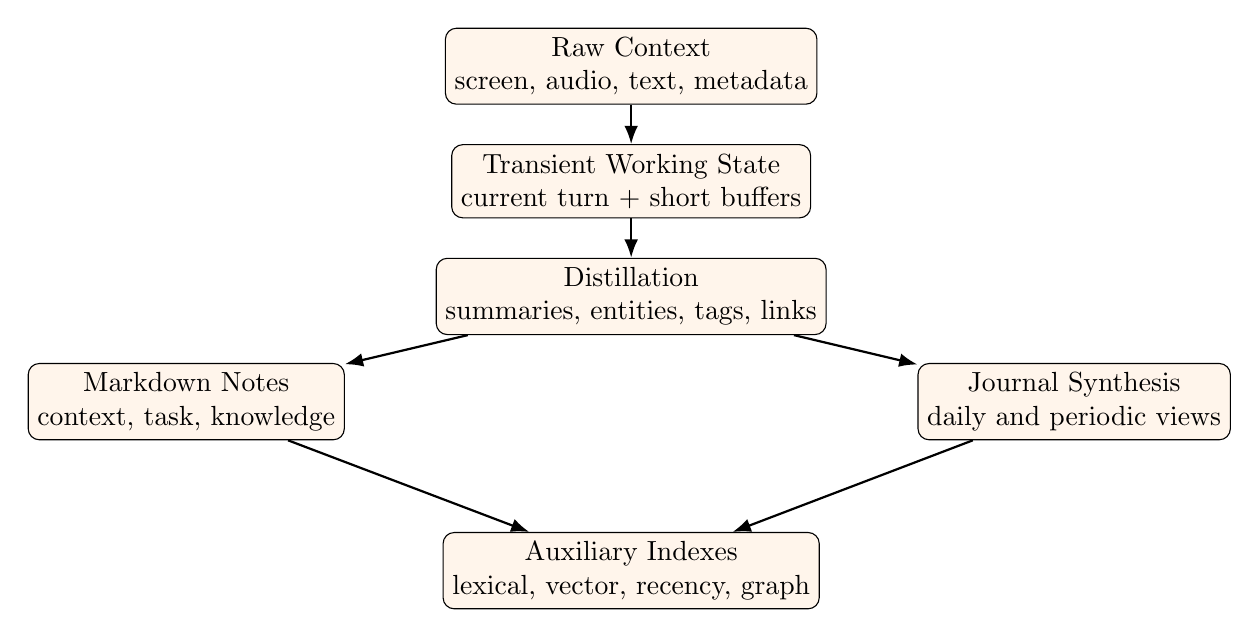
\begin{tikzpicture}[
  node distance=5mm,
  box/.style={draw, rounded corners, align=center, minimum height=7mm, minimum width=30mm, fill=orange!8},
  arrow/.style={-Latex, thick}
]
\node[box] (raw) {Raw Context\\screen, audio, text, metadata};
\node[box, below=of raw] (transient) {Transient Working State\\current turn + short buffers};
\node[box, below=of transient] (distill) {Distillation\\summaries, entities, tags, links};
\node[box, below left=of distill, xshift=-8mm] (notes) {Markdown Notes\\context, task, knowledge};
\node[box, below right=of distill, xshift=8mm] (journal) {Journal Synthesis\\daily and periodic views};
\node[box, below=of distill, yshift=-20mm] (indexes) {Auxiliary Indexes\\lexical, vector, recency, graph};

\draw[arrow] (raw) -- (transient);
\draw[arrow] (transient) -- (distill);
\draw[arrow] (distill) -- (notes);
\draw[arrow] (distill) -- (journal);
\draw[arrow] (notes) -- (indexes);
\draw[arrow] (journal) -- (indexes);
\end{tikzpicture}
}
\caption{Memory lifecycle in LAWRENCE. Raw capture is transient by default; durable Markdown artifacts and auxiliary indexes are produced through distillation.}
\label{fig:memoryloop}
\end{figure}

\subsection{Linking and Neighborhoods}
LAWRENCE does not treat memory as a bag of independent notes. Links matter. A note can be relevant because it mentions the same entities, because it is semantically close, because it was active recently, or because it lies in the local neighborhood of another already-recalled note. This graph-aware view is one reason a Zettelkasten-style substrate is preferable to a flat log.

For candidate notes $n_i$ and $n_j$, the system can assign a link score
\begin{equation}
\label{eq:link}
\begin{aligned}
S_{\mathrm{link}}(n_i,n_j) =\;&
\lambda_1 \cos(E_i,E_j) +
\lambda_2 \mathrm{Jaccard}(\mathcal{E}_i,\mathcal{E}_j) \\
&+
\lambda_3 R_{\mathrm{time}}(i,j) +
\lambda_4 R_{\mathrm{thread}}(i,j),
\end{aligned}
\end{equation}
where $E_i$ and $E_j$ are note embeddings, $\mathcal{E}_i$ and $\mathcal{E}_j$ are entity sets, $R_{\mathrm{time}}$ is temporal proximity, and $R_{\mathrm{thread}}$ measures whether the notes belong to the same ongoing activity cluster. A directed or undirected link is created when $S_{\mathrm{link}}$ exceeds a configured threshold. This gives the Zettelkasten graph a formal basis instead of relying only on ad hoc tag overlap.

\section{Retrieval as Evidence Gathering}
Retrieval in LAWRENCE is not an isolated retrieval-augmented generation module in the usual sense \cite{lewis2020rag}. It is one part of a broader evidence-gathering process. The assistant does not merely retrieve documents and then let one model answer from them. It combines multiple evidence streams that arrive in parallel.

The retrieval bundle for a turn may include:

\begin{itemize}
\item recent thread fragments,
\item recent context logs,
\item lexical matches,
\item semantic or vector hits,
\item graph-neighborhood expansions,
\item journal fragments,
\item web evidence when the web branch is active,
\item provenance markers for every item.
\end{itemize}

Hybrid retrieval matters because each method solves a different failure mode. Lexical retrieval preserves exact terminology. Vector similarity generalizes across wording. Recency keeps the assistant anchored to the current thread. Graph neighborhoods preserve task continuity. Together they produce a much stronger context bundle than any single method alone. Auxiliary vector indexing can be implemented through tools such as FAISS \cite{johnson2021faiss}, but the conceptual point is more important than the specific library: retrieval must respect semantics, continuity, and structure at the same time.

\subsection{Formal Retrieval Scoring}
For a candidate durable note $n$ and current turn state $t$, LAWRENCE can define the retrieval utility
\begin{equation}
\label{eq:retrieval}
\begin{aligned}
S_{\mathrm{ret}}(n \mid t) =\;&
\beta_\ell L(n,t) +
\beta_v V(n,t) +
\beta_g G(n,t) \\
&+
\beta_r R(n,t) +
\beta_h H(n,t) -
\beta_p P(n,t),
\end{aligned}
\end{equation}
where $L$ is lexical similarity, $V$ is semantic similarity, $G$ is graph proximity to already-relevant notes, $R$ is recency, $H$ is task or thread continuity, and $P$ is a privacy or routing penalty applied when an otherwise relevant note should not be surfaced in a given mode. Each term is normalized to a compatible range. The negative penalty term is useful because relevance alone is not enough; retrieval must also respect the current privacy and presentation state.

\subsection{Retrieval Bundle Definition}
The retrieval bundle for turn $t$ is not just a top-$k$ note list. It is a structured evidence package:
\begin{equation}
\label{eq:bundle}
\begin{aligned}
\mathcal{B}_t =\;&
\mathcal{R}^{\mathrm{recent}}_t \cup
\mathrm{TopK}_{n \in V}(S_{\mathrm{ret}}(n \mid t), K_m) \\
&\cup\ \mathrm{Expand}_h(\mathcal{L}_t, K_g) \cup
\mathcal{J}_t \cup
\mathcal{W}_t,
\end{aligned}
\end{equation}
where $\mathcal{R}^{\mathrm{recent}}_t$ is the recent conversational and thread context, $V$ is the durable note set, $\mathcal{L}_t$ is a set of local graph seeds, $\mathrm{Expand}_h$ returns up to $K_g$ graph-neighborhood notes within hop depth $h$, $\mathcal{J}_t$ is a set of relevant journal fragments, and $\mathcal{W}_t$ is the optional web-evidence bundle when the web branch is enabled by policy.

This definition matters because the reasoning layer should know what kind of evidence it is receiving. A recent-thread fragment does not carry the same semantics as a linked historical note or a web search result. By preserving the bundle as a typed evidence structure, LAWRENCE can maintain provenance, apply different confidence rules, and prevent web results from silently overwhelming local memory.

\section{Provider Gateway and Replaceable Runtime Backends}
The project is intentionally model-agnostic at the orchestration layer. That does not mean every backend is equal; it means the kernel should not need provider-specific branches just to perform its own duties. LAWRENCE therefore isolates inference backends behind a gateway contract.

The gateway has two jobs. First, it normalizes access to local and optional cloud model endpoints. Second, it makes routing decisions based on capability, health, latency, and policy. A fast local model may be good enough for immediate continuity. A larger or slower model may be appropriate for deferred reasoning. If one provider fails, the gateway should be able to fall back without forcing the orchestrator to understand transport details.

In the current implementation path, the primary local runtime is llama.cpp \cite{llamacpp}, the secondary local option is LM Studio, and OpenAI-compatible or Gemini-style cloud endpoints remain optional and policy-gated. This arrangement is a practical implementation choice, not a conceptual constraint. The project architecture is defined by the gateway boundary, not by loyalty to one runtime.

\section{Workflow and Tool Integration}
Modern assistants are often judged by what external systems they can call. LAWRENCE supports tool and workflow integration, but it does so carefully. Tool use is treated as one evidence and action branch among several, not as the definition of the assistant.

The current project path uses n8n Community Edition \cite{n8n} as a visible workflow layer. That choice is practical for three reasons. First, it offers a node-based editor that makes the external flows inspectable. Second, it allows web retrieval, note ingestion, local model calls, journal synthesis, and approval gates to be composed without embedding every integration detail into the kernel. Third, it lets the project demonstrate agentic behavior while keeping the assistant semantics in the kernel itself.

This distinction matters. n8n is not the brain. It is a replaceable workflow surface. The kernel still decides what a turn is, what evidence exists, what policy applies, and how outputs are merged.

Tool use follows the proposal model. A \emph{ToolActionProposal} includes the intended tool, arguments, risk level, whether confirmation is required, and the policy basis for the proposal. That structure is important because it separates planning from execution and keeps future actuation auditable.

\section{Privacy, Policy, and Local Control}
Any system that can inspect screen context, hear audio, call tools, and optionally reach the web can become irresponsible unless privacy controls are designed into the architecture from the beginning. LAWRENCE treats the policy layer as a first-class subsystem, not as a preferences page tacked on later.

\subsection{Assets and Trust Boundaries}
The primary assets in LAWRENCE are not only model prompts and outputs. They include raw screen and audio buffers, distilled context logs, long-term Markdown notes, workflow payloads, provider prompts, tool credentials, and any actuation privileges the system may hold. These assets cross different trust boundaries during a turn, and the architecture should make those boundaries explicit.

\begin{figure}[t]
\centering
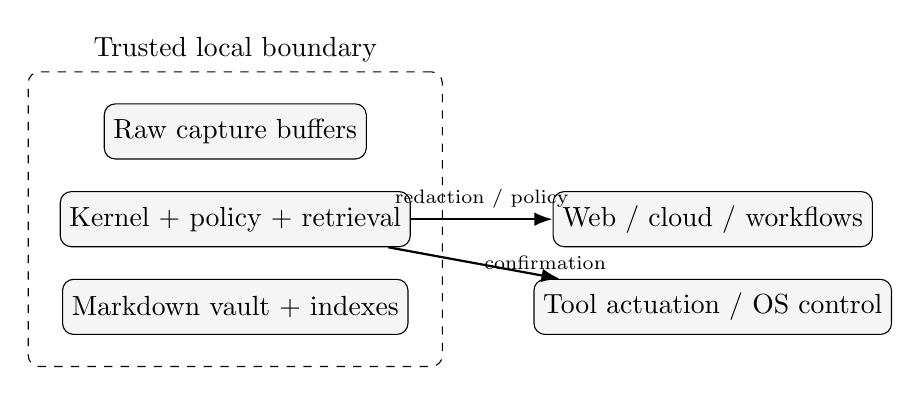
\begin{tikzpicture}[
  node distance=4mm and 8mm,
  comp/.style={draw, rounded corners, minimum width=29mm, minimum height=7mm, align=center, fill=gray!8},
  bound/.style={draw, dashed, rounded corners, inner sep=4mm},
  arrow/.style={-Latex, thick}
]
\node[comp] (raw) {Raw capture buffers};
\node[comp, below=of raw] (core) {Kernel + policy + retrieval};
\node[comp, below=of core] (vault) {Markdown vault + indexes};
\node[comp, right=18mm of core] (out) {Web / cloud / workflows};
\node[comp, below=of out] (act) {Tool actuation / OS control};
\node[bound, fit=(raw)(core)(vault), label=above:{Trusted local boundary}] (local) {};
\draw[arrow] (core) -- node[above, font=\scriptsize] {redaction / policy} (out);
\draw[arrow] (core) -- node[right, font=\scriptsize] {confirmation} (act);
\end{tikzpicture}
\caption{Trust boundaries in LAWRENCE. Raw capture, policy enforcement, and durable memory remain inside the local boundary; outbound retrieval and actuation cross explicit control boundaries.}
\label{fig:trust}
\end{figure}

The main trust boundaries are therefore: $(i)$ the raw-capture boundary between live inputs and the transient working set, $(ii)$ the durable-memory boundary between transient state and long-lived Markdown artifacts, $(iii)$ the outbound boundary between local reasoning and remote web or cloud systems, and $(iv)$ the actuation boundary between proposal and actual tool or operating-system control. These boundaries are more important than any individual model choice because they define where mistakes become serious.

The policy layer governs at least the following questions.

\begin{itemize}
\item Is microphone capture enabled?
\item Is screen capture enabled, and at what fidelity?
\item How long may raw buffers be retained?
\item Is web retrieval allowed for this mode or turn?
\item Is cloud inference allowed, and what must be redacted first?
\item Which tools can be proposed or executed?
\item When is explicit confirmation mandatory?
\end{itemize}

This policy mediation is especially important because LAWRENCE is personal-use-first. There is no default telemetry story that shifts trust to a remote vendor. The user must instead be able to inspect local memory, local logs, and local action trails.

\subsection{Threat Model}
The threat model for LAWRENCE is not primarily about nation-state adversaries or hostile enterprise networks. It is about realistic misuse and failure modes in a personal assistant that sees sensitive local context. These include prompt injection from observed content, accidental over-retention of raw capture, unintended disclosure through remote providers, unsafe tool execution, connector compromise, and silent feedback loops between generated content and later retrieval.

\begin{table}[t]
\caption{Representative threat classes and architectural controls}
\label{tab:threats}
\centering
\begin{tabular}{p{0.28\columnwidth} p{0.62\columnwidth}}
\toprule
\textbf{Threat class} & \textbf{Primary controls} \\
\midrule
Prompt injection from screen or web content & provenance tracking, tool-use separation, confirmation before actuation, policy-gated external calls \\
Accidental raw-data over-retention & transient buffers with TTL, explicit distillation thresholds, durable-write policy checks \\
Remote data leakage & local-first default, redaction before outbound calls, cloud disable switch, per-turn policy state \\
Unsafe tool execution & proposal/action split, risk levels, user confirmation, local audit trail \\
Workflow or connector drift & least-privilege connector boundaries, health checks, reproducible configs, local logs \\
Hidden ML feedback loops & retrieval provenance, evaluation loops, replay-based audits, operational monitoring \\
\bottomrule
\end{tabular}
\end{table}

\subsection{Formal Policy Gating}
For an outbound or state-changing operation $o$ during turn $t$, a simplified admissibility rule can be expressed as
\begin{equation}
\label{eq:policy}
\mathrm{Allow}(o,t) =
C(o,t) \land M(o,t) \land R(o,t) \land B(o,t) \land H(o,t),
\end{equation}
where $C$ is user consent, $M$ is mode and policy compatibility, $R$ is redaction sufficiency, $B$ is boundary compliance, and $H$ is human confirmation when required. Read-only local retrieval may satisfy $H$ automatically, whereas web calls, cloud inference, or tool execution may not. This equation is intentionally simple, but it clarifies that relevance alone never authorizes an operation.

\section{Implementation Architecture}
The conceptual model above becomes concrete through a specific implementation architecture. The purpose of this section is to explain why the project uses the current stack, not to argue that the stack is the only valid possibility.

\subsection{Desktop-First Host Surface}
LAWRENCE currently adopts a desktop-first host strategy built around Tauri \cite{tauri}. This decision follows from the project's need for overlays, low-level hooks, and local-runtime control. A browser-only host would make some of those integrations harder at the stage where the project most needs them. Tauri provides a pragmatic middle ground: the UI can use web technologies while the system can still access native integration through Rust.

\subsection{Assistant Kernel}
The kernel is implemented in Python using FastAPI and asynchronous task orchestration. Python is an effective choice for the kernel because the work is coordination-heavy: provider adapters, retrieval, memory writing, policy enforcement, and workflow calls are easier to iterate in Python than in a fully native stack. The kernel remains the single authority for turn lifecycle and contract enforcement.

\subsection{System Hooks}
System hooks are separated from the kernel and handled through native helper boundaries, currently intended to be Rust-based. This is important because microphone access, screen capture, hotkeys, and window inspection have different operational and packaging concerns than the assistant logic itself.

\subsection{Speech Path}
Speech input can be served by local speech-to-text runtimes derived from Whisper \cite{radford2022whisper}. Voice output is intentionally split into a reliable baseline TTS path and an optional expressive styling layer. This reflects the project's scope discipline: intelligibility and responsiveness matter more than theatrical prosody in the first serious version.

\subsection{Connector and Workflow Layer}
The connector layer contains n8n today and can contain MCP or other adapters later. The key point is that connectors live outside the core assistant semantics. This prevents rapid integration churn from destabilizing the kernel.

\begin{table}[t]
\caption{Representative implementation mapping for LAWRENCE v0.1}
\label{tab:implmap}
\centering
\begin{tabular}{p{0.28\columnwidth} p{0.62\columnwidth}}
\toprule
\textbf{Subsystem} & \textbf{Current implementation choice} \\
\midrule
Desktop host & Tauri + React + Vite \\
Kernel & Python + FastAPI + async orchestration \\
Hooks & Rust-native helper boundary \\
Local LLM runtime & llama.cpp primary, LM Studio alternate \\
Workflow layer & n8n Community Edition \\
Durable memory & Markdown vault with frontmatter \\
Retrieval acceleration & lexical, vector, recency, graph sidecars \\
Policy layer & local config + per-turn policy state \\
\bottomrule
\end{tabular}
\end{table}

\section{Core Algorithms and Contracts}
The architecture becomes clearer when stated algorithmically. Algorithm~\ref{alg:turn} describes the central turn-processing routine.

\begin{algorithm}[t]
\caption{Parallel turn processing in LAWRENCE}
\label{alg:turn}
\begin{algorithmic}[1]
\Procedure{ProcessTurn}{$event$}
\State $snapshot \gets \mathrm{FreezeContextSnapshot}(event)$
\State $facets \gets \mathrm{SelectFacets}(snapshot, policy)$
\ForAll{$f \in facets$ \textbf{in parallel}}
\State launch $\mathrm{RunFacet}(f, snapshot)$ with budget and timeout
\EndFor
\State $results \gets [\ ]$
\While{fast deadline not exceeded}
\State $r \gets \mathrm{NextCompletedFacetResult}()$
\If{$r.context\_version = snapshot.context\_version$}
\State Append($results, r$)
\EndIf
\If{MeetsFastThreshold($results$)}
\State $decision \gets \mathrm{MergeImmediate}(snapshot, results)$
\State $\mathrm{EmitImmediateResponse}(decision)$
\State \textbf{break}
\EndIf
\EndWhile
\State $late \gets \mathrm{CollectRemainingFacetResults}(snapshot.context\_version)$
\State $final \gets \mathrm{MergeDeferred}(snapshot, results \cup late)$
\State $\mathrm{PersistDistillationsAndNotes}(final)$
\State $\mathrm{EmitDeferredAddendumIfUseful}(final)$
\EndProcedure
\end{algorithmic}
\end{algorithm}

The algorithm makes the project semantics explicit. There is one turn, one snapshot, many facets, one merge boundary, and potentially two user-visible emissions: immediate and deferred.

Algorithm~\ref{alg:distill} shows the simplified note distillation flow.

\begin{algorithm}[t]
\caption{Distillation, linking, and raw-data expiry}
\label{alg:distill}
\begin{algorithmic}[1]
\Procedure{DistillAndLink}{$turn, evidence$}
\State $record \gets \mathrm{SummarizeTransientContext}(turn, evidence)$
\State $entities \gets \mathrm{ExtractEntities}(record)$
\State $candidates \gets \mathrm{RetrievePotentialLinks}(entities, record.summary)$
\State $scored \gets \mathrm{ScoreBySimilarityRecencyThreadAndGraph}(candidates, record)$
\State $links \gets \mathrm{KeepAboveThreshold}(scored)$
\State $note \gets \mathrm{BuildMarkdownNote}(record, entities, links)$
\State $\mathrm{WriteNote}(note)$
\State $\mathrm{ExpireRawBuffersAccordingToPolicy}(turn)$
\EndProcedure
\end{algorithmic}
\end{algorithm}

The main contracts that stabilize the architecture are summarized in Table~\ref{tab:contracts}.

\begin{table}[t]
\caption{Primary inter-module contracts}
\label{tab:contracts}
\centering
\small
\begin{tabular}{>{\raggedright\arraybackslash}p{0.25\columnwidth} >{\raggedright\arraybackslash}p{0.65\columnwidth}}
\toprule
\textbf{Contract} & \textbf{Role} \\
\midrule
TurnContextSnapshot & Frozen turn reference shared by all facets. \\
FacetResult & Standard evidence record with confidence, citations, actions, and context version. \\
MergeDecision & Immediate response, deferred allowance, overlays, follow-ups, and structured outputs. \\
ToolActionProposal & Proposed action with risk and confirmation metadata. \\
DistillationRecord & Mapping from transient source to durable artifact and retention policy. \\
LLMProviderAdapter & Capability and generation surface for replaceable inference backends. \\
\bottomrule
\end{tabular}
\end{table}

\section{Supervisory Control, MLOps, and Search-Augmented Orchestration}
The architecture described so far is sufficient for a coherent assistant, but not yet for a self-stabilizing one. As the number of providers, workflows, triggers, and note-writing paths grows, LAWRENCE benefits from a supervisory layer that watches the watcher. This is where MLOps-style recurrent evaluation, PID-like control, Petri-net reasoning, and bounded tree search can help. These mechanisms should be understood as control-plane tools rather than as the product's visible personality.

\subsection{MLOps and Recurrent Evaluation Loops}
Real machine learning systems accumulate technical debt through hidden feedback loops, brittle dependencies, and glue logic sprawl \cite{sculley2015debt}. LAWRENCE is especially exposed to this risk because its outputs affect later inputs: generated notes change retrieval, retrieved notes change answers, and answers may influence what the user does next. A useful MLOps layer for LAWRENCE should therefore track more than model accuracy. It should monitor retrieval usefulness, note growth rate, confirmation overruns, tool proposal acceptance, latency distributions, stale-result rates, and memory drift. These metrics form recurrent operational loops that drive retuning and regression testing rather than being collected for telemetry.

\subsection{PID-Like Runtime Budget Control}
Although LAWRENCE is not a physical control system, some of its behaviors can be stabilized using PID-like feedback controllers \cite{astrom1995pid}. Let $y_t$ denote observed runtime behavior such as fast-loop latency, timeout rate, memory-write rate, or web-branch cost, and let $y^\star$ denote the desired operating point. A control error is
\begin{equation}
e_t = y^\star - y_t.
\end{equation}
The supervisor can then update a control vector
\begin{equation}
\label{eq:pid}
u_t = \mathrm{clip}\left(
K_P e_t +
K_I \sum_{\tau=0}^{t} e_\tau +
K_D (e_t - e_{t-1})
\right),
\end{equation}
where $u_t$ parameterizes facet deadlines, screenshot sampling rate, retrieval depth, web-branch aggressiveness, or slow-loop budget. The point is not to mimic industrial control literally. The point is to use feedback to keep the assistant inside a stable operating envelope on limited hardware.

\subsection{Petri-Net View of Concurrency and Safety}
Petri nets are a useful formalism for reasoning about concurrency, reachability, and enabled transitions in event-driven systems \cite{murata1989petri}. LAWRENCE is a strong candidate for such a model because it already behaves like a network of concurrent transitions over resource tokens. A token can represent an active snapshot, policy approval, write permission, tool confirmation, or merge readiness. A transition can represent facet dispatch, evidence merge, note commit, or tool execution.

This framing is practically useful. It allows the system to express invariants such as: no tool execution without both a policy token and a user-confirmation token; no durable write without a distillation token; no merge-finalization without at least one valid facet result. Petri-net reasoning is therefore a good fit for a future supervisory layer that needs to verify legal state transitions while still allowing parallel execution.

\subsection{MDP and MuZero-Like Search for the Slow Loop}
The slow loop can also be viewed as a finite-horizon decision process over partially known assistant states. This admits a Markov decision process interpretation \cite{puterman1994mdp} in which the assistant state includes the snapshot, current evidence bundle, open questions, candidate tool calls, and partially formed responses. A search policy over that state can decide whether the next best move is to expand retrieval, ask a clarifying question, invoke the web branch, compare candidate answers, or terminate with a refined response.

MuZero is relevant here not because LAWRENCE should reproduce game-playing infrastructure, but because MuZero demonstrates how useful planning can emerge from a learned model without requiring a perfect simulator \cite{schrittwieser2020muzero}. A bounded MuZero-like or PUCT-style tree expansion can help the slow loop evaluate candidate refinement paths:
\begin{equation}
\label{eq:puct}
a^\star = \arg\max_a \left[
Q(s,a) + c_{\mathrm{puct}} P(s,a)\frac{\sqrt{N(s)}}{1+N(s,a)}
\right],
\end{equation}
where $Q$ estimates downstream utility, $P$ is a prior over expansions, and $N$ counts visits. In LAWRENCE, actions are not chess moves; they are candidate next reasoning steps such as ``expand graph neighborhood,'' ``retrieve web evidence,'' ``synthesize task note,'' or ``finalize answer.'' This type of search should remain tightly bounded in branch factor and depth so that it improves quality without violating the project's local-hardware constraints.

\subsection{Why These Mechanisms Belong in the Control Plane}
PID-like controllers, Petri nets, recurrent MLOps loops, and MuZero-like bounded search are powerful precisely because they operate above the individual model call. They help regulate the assistant as a system of interacting parts. In LAWRENCE they should therefore be used to supervise budgets, legal transitions, regression quality, and deeper optional planning, not to replace the core kernel or to obscure the simple turn model.

\section{Operational Envelope and Failure Behavior}
LAWRENCE is intended to run under meaningful resource constraints. For that reason, the system prefers bounded work over maximal work. Per-facet deadlines, token budgets, and priority scheduling are not optimizations added later; they are part of the design.

The failure philosophy is similarly explicit.

\begin{itemize}
\item If the web branch fails, the assistant should still answer from local evidence.
\item If the slow loop is late, the fast-loop answer should stand.
\item If note writing fails, the system should preserve a retry path instead of silently discarding context.
\item If one provider is unavailable, the gateway should route to another or decline according to policy.
\item If a tool action is unsafe or blocked, the system should return a proposal-only result.
\end{itemize}

This failure model is a direct consequence of the parallel-facet design. The system degrades branch by branch rather than failing all at once.

\section{Discussion}
LAWRENCE is best understood as a synthesis of three ideas that are usually kept apart. The first is the chatbot-like conversational surface. The second is the personal knowledge system, represented here by linked Markdown notes. The third is the agentic runtime with tools and workflows. The project is not merely combining these three components side by side. It is integrating them around one turn model and one kernel.

That integration creates tradeoffs. Markdown memory is transparent, but it requires disciplined distillation and indexing. Parallel facets improve responsiveness, but they increase merge complexity. Desktop-first integration improves practical capability, but it introduces packaging work. Strong policy mediation makes the system safer, but it also forces the project to be explicit about what many AI demos conveniently ignore.

These tradeoffs are acceptable because the system is not trying to be the easiest demo. It is trying to be a serious substrate for a privacy-aware personal assistant that grows durable knowledge.

\section{Limitations and Extensions}
Several subsystems are architecturally defined but not yet fully realized in depth. These include live microphone and screen watcher wiring, a stronger retrieval stack with mature BM25 and ANN support, a full recommendation subsystem, more sophisticated slow-loop critique and bounded recursion, and a more mature speech output path. Importantly, these are implementation-depth gaps rather than unresolved conceptual questions.

Likewise, the current implementation path intentionally favors a narrow set of well-integrated backends: desktop-first Tauri hosting, Python kernel orchestration, llama.cpp for local inference, and n8n for visible workflows. Broader backend coverage can come later as long as the core contracts remain stable.

\section{Conclusion}
LAWRENCE is a local-first watcher-assistant architecture built around one assistant kernel with many simultaneous internal facets. Its core claim is that useful assistance requires more than generating a strong answer to the current prompt. It requires contextual sensing, explicit time and thread awareness, durable inspectable memory, concurrent evidence gathering, optional tool and web branches, and a clean separation between immediate response and slower refinement. By storing durable knowledge as linked Markdown, routing inference through replaceable backends, and placing privacy policy at the center of the design, LAWRENCE proposes a practical architecture for a personal multimodal assistant that remains understandable and controllable as it grows.

\balance
\bibliographystyle{IEEEtran}
\bibliography{LAWRENCE_v0_1_refs}

\end{document}
